%%% New implementation section 

\section{Monitor Implementation and Evaluation}

%% paragraph 1 -- goals
To evaluate the feasibility of our monitoring algorithm for safety-critical real-time systems we have built a real-time CAN monitor on an ARM Cortex-M4 development board. This allowed us to explore the necessary optimizations and features required to perform real-time checking of realistic safety policies.

%% paragraph 2 -- what we built

%% Embedded restrictions
Software for safety-critical embedded systems typically contains more strict design and programming model constraints than less critical software. Two important and common constraints for these systems are avoiding recursion and not using dynamic memory allocations. 
% dynamic memory alloc
Common safety-critical coding guidelines discourage or prohibit dynamic memory allocation to avoid memory leaks.
Because our specification language is bounded, we can avoid dynamic allocation in our \monitor implementation by statically allocating space for the maximum number of entries for our history structures and other temporary data structures.
% recursion
Recursion is also usually prohibited because it can be difficult to guarantee a maximum stack depth when using recursion. Although \monitor utilizes recursion extensively, we can implement \monitor using a traditional iterative traversal of the specification formulas instead.

\subsection{Hybrid Algorithm}
Our eager monitoring algorithm attempts to evaluate specification rules as soon as possible, but this requires checking trace properties which may not be fully reducible given the current trace. These unfinished formula reductions require extra computation time, and in practice the majority of the policy reductions performed by \monitor will be these eager reductions which may not fully reduce.

While early detection of violations can be useful, there are situations where eagerly checking an entire target specification may require more computation than is available from the monitor in a given period.

To enable the benefits of eager checking while avoiding the risks of losing real-time correctness, we have implemented a hybrid eager monitoring algorithm which performs non-eager (conservative) checking first and uses any spare time to eagerly check the remaining monitor residues.
%
Conservative \monitor monitoring is performed by only checking residues which are older than their formula delay, which guarantees that these residue will be reduced at their first evaluation.
%
Under our periodic sampling design, each step of conservative monitor only requires updating the history structures and checking a single residue (the oldest remaining one) for each specification policy.
%
This conservative check can be done quickly at each period, leaving any extra time until the next period for eager checking. This provides a conservative monitoring guarantee (\ie, the specification is checked within a known promptness delay) while also allowing the monitor to eagerly check as much of the specification as possible.

%As long as we know that the worst case execution time for message handing, incrementing the structures, and a single residue check is short enough to finish within a monitor period then we are guaranteed at least a conservatively correct and prompt output.

\begin{figure}[t]
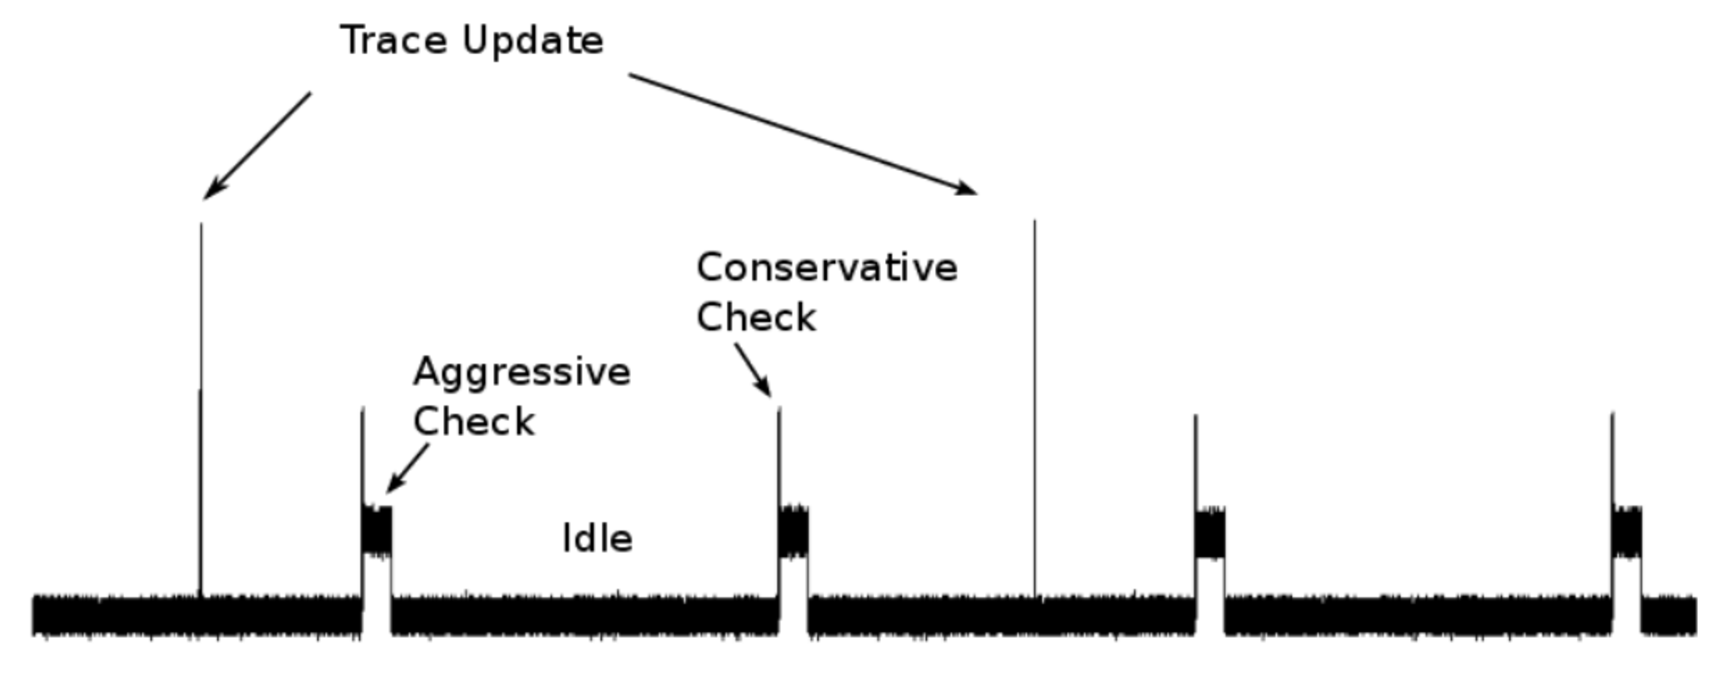
\includegraphics[width=4.5in]{img/scope_annotated_crop}
\caption{Oscilloscope capture of embedded monitor task execution \label{fig:arch:oscope}}
\end{figure}

We have implemented the hybrid monitoring algorithm in our embedded monitor. The monitor updates the history structures (shared between the conservative and eager checking) and performs a conservative check once every monitoring period. It then uses the idle time between periods to perform eager checking of any remaining unchecked specification properties.
%
Figure \ref{fig:arch:oscope} shows the execution of the embedded monitor instrumented to output the currently executing task to an oscilloscope. The residue checks run twice per trace update due to the monitor configuration used during the test, but this is not required for correct monitoring.
This task output was captured while monitoring the specification used in the case study (see Section \ref{sec:case_study} plus another 200 time-step \emph{eventually} rule which was never satisfied. 
%(guaranteeing an extra 200 eager residue checks every period). 
The rule never being satisfied means that at every step the monitor performed an eager check of all 200 residues for this rule at every step (i.e., since they were never satisfied, they could never be reduced early). 
Even with this excess computation there was still a large portion of extra idle time -- 23ms of the 25ms monitoring loop was spent idle. 
This shows the eager checking finished reasonably quickly and the monitor could handle much longer formula durations or more complex formulas before the execution time becomes bad enough to require the hybrid algorithm for correctness guarantees. 

\subsection{Case Study}
\label{sec:case_study}
This section reports our case study performing real-time monitoring of a CAN network for realistic safety properties. 
For this case study we have obtained CAN network logs from a series of robustness tests on the ARV which we have replayed on a test CAN bus for the monitor to check. 
This setup, %shown in Figure \ref{fig:replaySchem}, 
helps us show the feasibility of performing external bus monitoring on this class of system with real safety specifications.

%% removing, takes space and not that important
%\begin{figure}
%\centering
%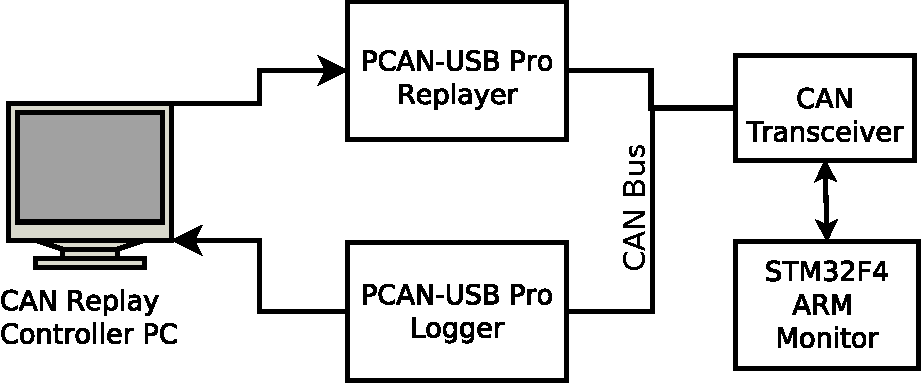
\includegraphics[width=3in]{img/replay_arch}
%\caption{CAN replay network setup \label{fig:replaySchem}}
%\end{figure}

%% paragraph 3 -- description of experiment 
%%% some of this is in para1, we should go over: specification, logs, etc
The logs contain both normal system operation as well as some operation under network-based robustness testing. During robustness testing, the testing framework can intercept targeted network messages on the bus and inject its own testing values. % could cite astaa here
A PC was connected to a PCAN-USB Pro \cite{PCAN-USBPro} device which provides a USB interface to two CAN connections. One CAN channel was used as the log re-player, while the other was used as a bus logger for analysis purposes.

%% paragraph 4 -- specification
Requirements documentation for this system was available, so we were able to build a monitoring specification based on actual system requirements.
The specification evaluated in the embedded monitor on the test logs are shown in Table \ref{tab:monspec}. This specification was derived from the system requirements based on the observable system state available in the testing logs. 



\begin{table}[t]
%\begin{tabular}{|p{3in}|l|}
\begin{tabular}{|l|p{4.5in}|}
\hline \multirow{2}{*}{Rule \#} & Informal Rule \\ & BMTL \\
\hline \multirow{2}{*}{0} & A feature heartbeat will be sent within every 500ms \\
& $\pred{HeartbeatOn} \rightarrow \LTLdiamond_{[0,500ms]} \pred{HeartBeat}$ \\
\hline \multirow{2}{*}{1} & The interface component heartbeat counter is correct \\
& $\pred{HeartbeatOn} \rightarrow \pred{HeartbeatCounterOk}$ \\
\hline \multirow{2}{*}{2} & The vehicle shall not transition from manual mode to autonomous mode \\
&  $\neg ((\LTLcircleminus_{[0,25ms]} \pred{IntManualState}) \wedge \pred{IntAutoStat})$\\
\hline \multirow{2}{*}{3} & The vehicle controller shall not command a transition from manual mode to autonomous mode \\
& $\neg ((\LTLcircleminus_{[0,25ms]} \pred{VehManualModeCmd}) \wedge \pred{VehAutoModeCmd})$\\
\hline \multirow{2}{*}{4} & The vehicle shall not transition from system off mode to autonomous mode \\ 
&  $\neg ((\LTLcircleminus_{[0,25ms]} \pred{IntSDState}) \wedge \pred{IntAutoStat})$\\
\hline \multirow{2}{*}{5} & The vehicle controller shall not command a transition from system off mode to autonomous mode \\
& $\neg ((\LTLcircleminus_{[0,25ms]} \pred{VehSDModeCmd}) \wedge \pred{VehAutoModeCmd})$\\
% warn was at 200ms
\hline
\end{tabular}
\caption{Case study monitoring specification \label{tab:monspec}}
\end{table}

Rule \#0 is a heartbeat detection which ensures that the interface component is still running (essentially a watchdog message). Rule \#1 is a second component of this check. The system's heartbeat message contains a single heartbeat status bit which we checked directly in Rule \#0, but the message also has a rolling counter field. We use the \sfmap to ensure that this counter is incrementing correctly and output this check as the $\pred{HeartbeakOk}$ predicate which is checked in Rule \#1.
We also checked for illegal state transitions. Rules \#2 through \#5 check both for illegal transition commands from the vehicle controller and actual illegal state transitions in the interface component.

%% move hybrid algorithm explanation here maybe?

\subsection{Monitoring Results}
Monitoring the test logs with the above specification resulted in identifying two real violations as well as some false positive violation detections caused by the testing infrastructure.
%
% covering all three possible violation types. One was a false positive
Three different types of heartbeat violations were identified after inspecting the monitor results, some actual violations and some false-positives caused by the testing infrastructure. We also identified infrastructure-caused false-positive violations of the transition rules.

\begin{figure}[t]
		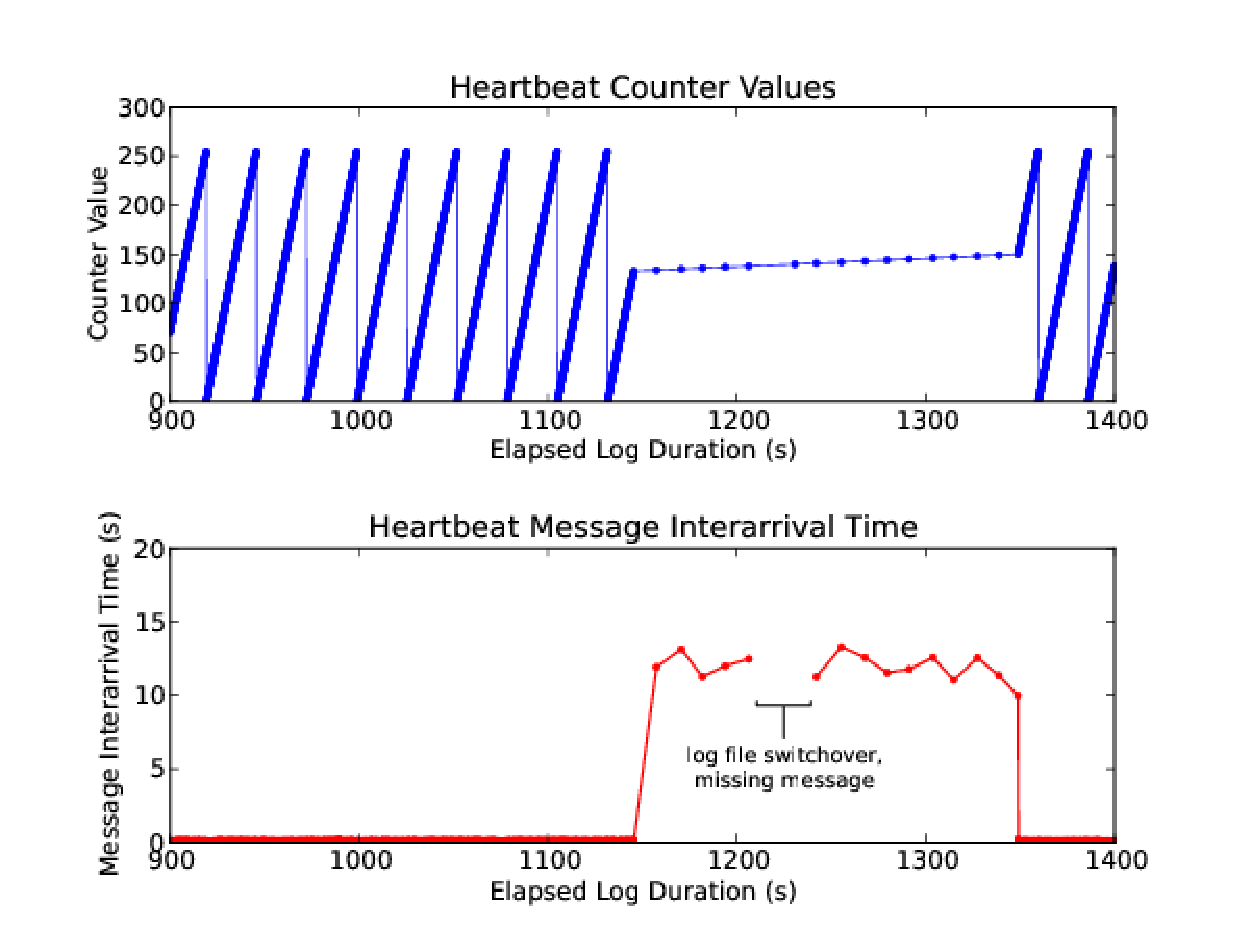
\includegraphics[width=4.5in]{img/hb1}
		\caption{Heartbeat counter values over time}
		\label{fig:hb_arrival}
\end{figure}

\paragraph{Specification violations.}
% missing hb message
The first violation is a late heartbeat message. In one of the robustness testing logs the heartbeat message was not sent on time, which is clearly a heartbeat violation. Figure \ref{fig:hb_arrival} shows the heartbeat counter values and the inter-arrival time of the heartbeat messages over time for this violation. We can see here that the heartbeat counter did in fact increment in a valid way, just too slowly. 
% bad status
The second violation is on-time heartbeat status message but the heartbeat status field is 0. 
We do not know from the available documentation whether a bad status in an on-time message with a good counter is valid or not. So without more information we cannot tell whether these violations are false positives or not. This is worthy of further investigation.


\begin{figure}[t]
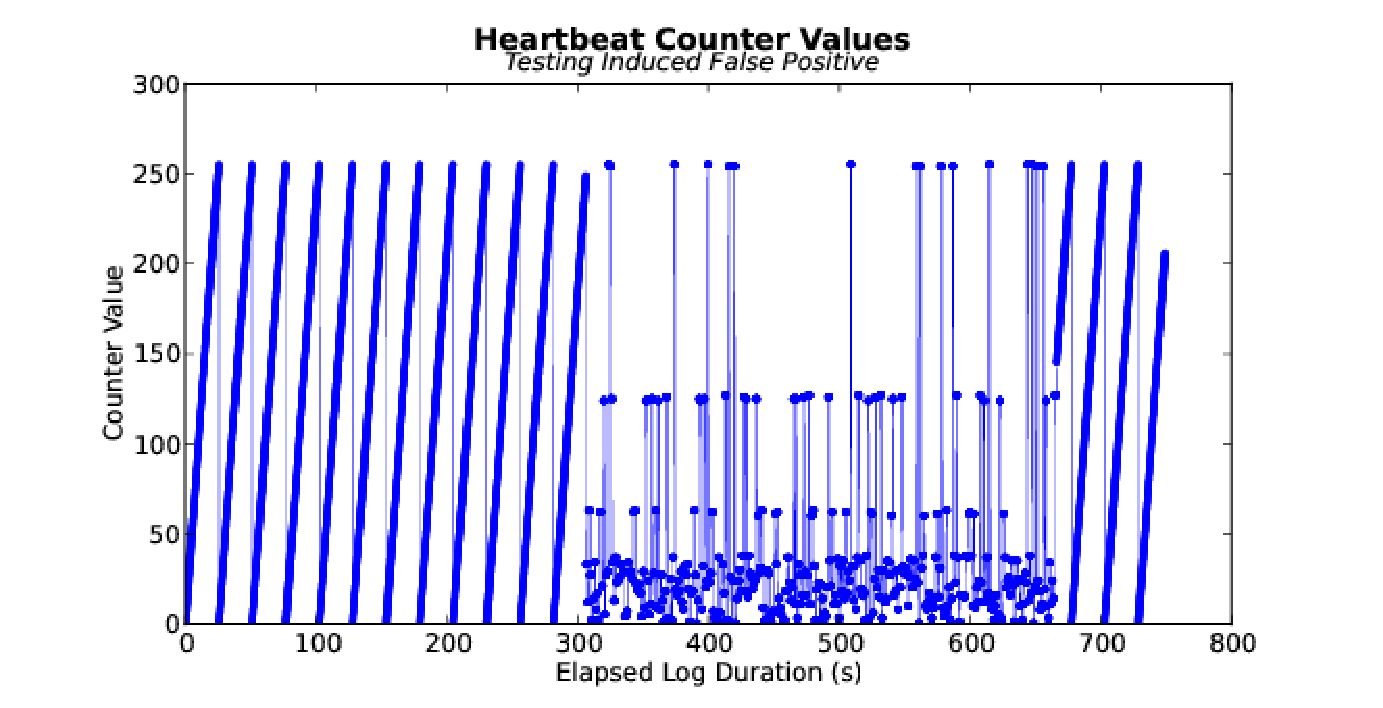
\includegraphics[width=4.5in]{img/hb2}
\caption{Bad heartbeat counter values \label{fig:hb_badcounter}}
\end{figure}

\paragraph{False-positive violations.}
% bad counter
The last type of heartbeat violation is a bad counter. 
We have defined a good counter as one which increments by one every message up to its maximum (255 in this case) before wrapping back to zero.
Every consecutive heartbeat status message must have an incremented heartbeat counter or a violation will be triggered. Figure \ref{fig:hb_badcounter} shows the counter value history for one of the traces with a heartbeat violation caused by a bad counter value.
%
%@EDIT describe robustness testing, define these false positives like the talk?
Further inspection of this violation showed that the bad counter values were sent by the testing framework rather than the actual system. In this case, the network traffic the monitor is seeing is not real system state but actually it is messages being injected by the testing framework. This is not a real violation (since the violating state is not the actual system state), and so we consider this a false positive violation.



The monitor also reported violations of the legal transition rules, but these, similar to the heartbeat counter violation, also turned out to be false positives triggered by message injections by the robustness testing harness. Since the monitor checks network state, if we perform testing that directly affects the values seen on the network (such as injection/interception of network messages) we may detect violations which are created by the testing framework rather than the system. 
Information about the test configurations can be used to filter out these types of false positives which arise from test-controlled state.
This type of filtering can be automated if the test information can be input to the monitor, either directly on the network (e.g., adding a message value to injected messages) or through a side-channel (i.e., building a testing-aware monitor).
